\documentclass[10pt,twocolumn,letterpaper]{article}

\usepackage{cvpr}
\usepackage{times}
\usepackage{epsfig}
\usepackage{graphicx}
\usepackage{amsmath}
\usepackage{amssymb}
\usepackage{gensymb}

% Include other packages here, before hyperref.

% If you comment hyperref and then uncomment it, you should delete
% egpaper.aux before re-running latex.  (Or just hit 'q' on the first latex
% run, let it finish, and you should be clear).
%\usepackage[pagebackref=true,breaklinks=true,letterpaper=true,colorlinks,bookmarks=false]{hyperref}

\cvprfinalcopy % *** Uncomment this line for the final submission

\def\cvprPaperID{****} % *** Enter the 3DV Paper ID here
\def\httilde{\mbox{\tt\raisebox{-.5ex}{\symbol{126}}}}

% Pages are numbered in submission mode, and unnumbered in camera-ready
%\ifcvprfinal\pagestyle{empty}\fi
\setcounter{page}{1}
\begin{document}

%%%%%%%%% TITLE
\title{Omni-directional stereo for 360$\degree$ 3D virual reality video}

\author{Prashanth Chandran\\
ETH Zurich\\
www.ethz.ch\\
{\tt\small chandranp@student.ethz.ch}
% For a paper whose authors are all at the same institution,
% omit the following lines up until the closing ``}''.
% Additional authors and addresses can be added with ``\and'',
% just like the second author.
% To save space, use either the email address or home page, not both
\and
Sasha Pagani\\
ETH Zurich\\
www.ethz.ch\\
{\tt\small paganis@student.ethz.ch}
\and
Julia Giger\\
ETH Zurich\\
www.ethz.ch\\
{\tt\small jgiger@student.ethz.ch}
}

\maketitle
%\thispagestyle{empty}

%%%%%%%%% ABSTRACT
\begin{abstract}
   The aim of our project is to produce omni-directional stereo images and videos, which are for example viewable in the Google Cardboard, similar to Anderson et al.~\cite{jump16}. The input for our pipeline are the images of a camera rig, which are stitched together for receiving omni-directional images. This process has to been carried out twice, once for the left and once for the right eye to get an omni-directional stereo image.
\end{abstract}

%%%%%%%%% BODY TEXT
\section{Introduction}

The stereo view of our eyes is created by fusing the image from the left eye with the one from the right eye. This enables us to perceive a stereo impression of the world. Therefore, to produce stereo videos, we need to capture synchronized videos from two cameras set apart at interpupillary distance (IPD), which denotes the distance between the two eyes and is on average about 6.4 cm. However, the goal of this project is not only to produce stereo, but omni-directional, which means 360$\degree$, videos. The first simple idea coming in mind to capture such videos is to place two omni-directional cameras with a distance of IPD. One issue with such an approach is that the two cameras will see each other, which is undesirable. However, the more important problem is that objects lying on the line between the two camera centers will have no disparity (see figure~\ref{two_360}). Disparity denotes the amount of shift in the image position between the left and the right eye. Therefore, this simple solution does not work and would not produce the desired omni-directional stereo videos.

The ideal solution would be to have a stereo image pair for every head orientation, for example one pair for each degree (see figure~\ref{wanted}). However, this would be a huge amount of images. The main idea is to approximate this optimal view by only capturing the central ray of each camera instead of the full image at each head orientation (see figure~\ref{approx}). Figure~\ref{ods} illustrates the extension of this approach to 360$\degree$.

\begin{figure}[t]
\begin{center}
   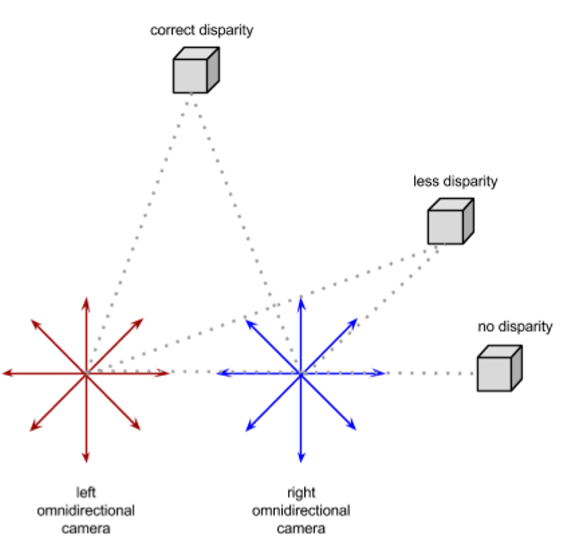
\includegraphics[width=0.8\linewidth]{pictures/two_360.png}
\end{center}
   \caption{Illustration of two 360$\degree$ cameras placed next to each other.}
\label{two_360}
\end{figure}

\begin{figure}[t]
\begin{center}
   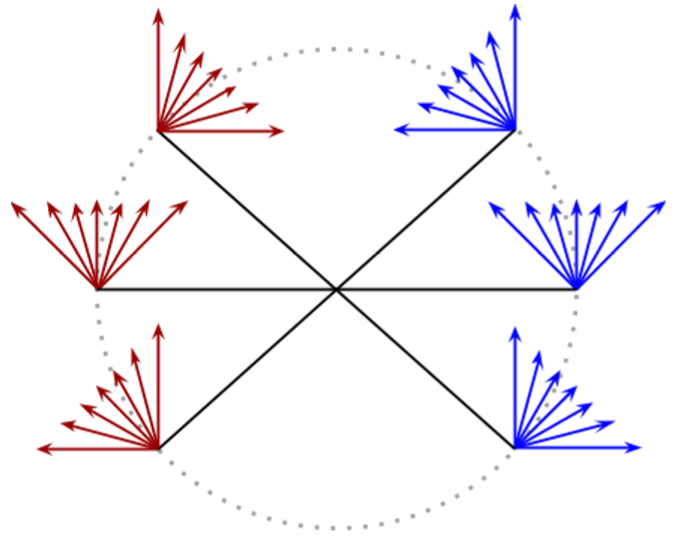
\includegraphics[width=0.5\linewidth]{pictures/wanted.png}
\end{center}
   \caption{This image shows the most optimal situation, where a full image is captured for each head direction. The red rays illustrate the left eye and the blue ones the left eye.}
\label{wanted}
\end{figure}

\begin{figure}[t]
\begin{center}
	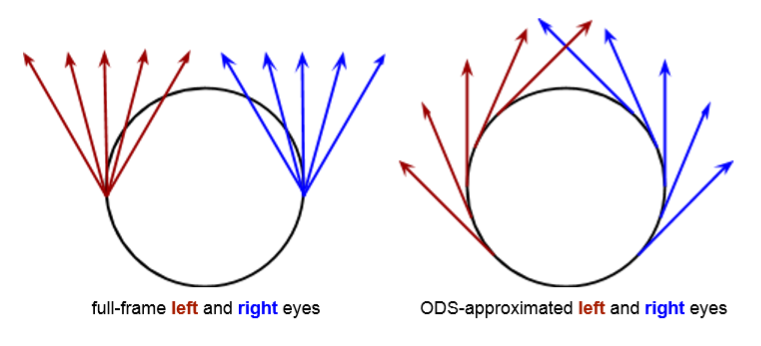
\includegraphics[width=0.8\linewidth]{pictures/approxi.png}
\end{center}
   \caption{The left image shows the rays for capturing the full image at one head direction. The right image illustrates the ODS approximation by using only the central ray of each camera position.}
\label{approx}
\end{figure}

\begin{figure}[t]
\begin{center}
   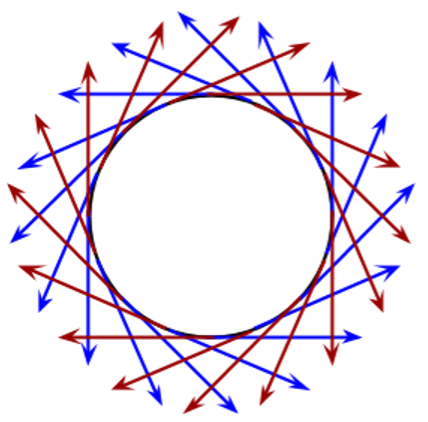
\includegraphics[width=0.5\linewidth]{pictures/ods.png}
\end{center}
   \caption{This image shows the ODS approximation for 360$\degree$. The red rays illustrates the left eye and the blue rays the right eye.}
\label{ods}
\end{figure}


%------------------------------------------------------------------------
\section{Related work}
The whole project is based on a paper by Anderson et al.~\cite{jump16}, where a system for viewing omni-directional stereo videos, called 'Jump', is introduced. Therefore, our main pipeline is the same as described in Anderson et al.~\cite{jump16}. However, we did not implement the sophisticated algorithm for the flow computation. We used a provided method of OpenCV for the flow estimation. Furthermore, we simplified the exposure correction and the composition step. For the implementation details, we also used the article~\cite{ods} by Google Inc.

%------------------------------------------------------------------------
\section{Work subdivision}

%------------------------------------------------------------------------
\section{Method}
An overview of our pipeline can be found in figure~\ref{pipeline}. The inputs are 10 synchronized videos from a camera rig. The first step is the calibration of the different cameras of the rig, which includes the computation of the intrinsics and extrinsics of each camera. The next step is the optical flow estimation between the neighboring camera pairs. For having nice transitions in the final ODS stitch, an exposure correction between neighboring image pairs is applied. Based on the computed flow values, the view interpolation between the images is calculated and they are stitched together as a final step, which results in the desired ODS video.

\begin{figure}[t]
\begin{center}
   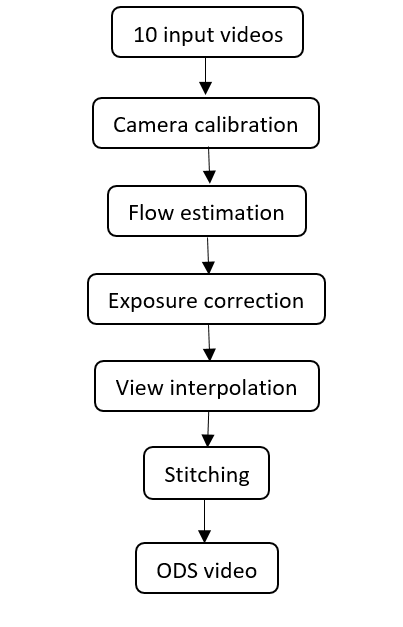
\includegraphics[width=0.3\linewidth]{pictures/pipeline.PNG}
\end{center}
   \caption{Overview of the pipeline.}
\label{pipeline}
\end{figure}

\subsection{Camera calibration}
Additionally to the dataset, consisting of 10 videos, we received a calibration file from our supervisor, which contained the calibration data for each camera. This calibration data consists of the intrinsic and relative extrinsic of each camera. For the computation in the later stages of our pipeline, we also needed the absolute extrinsics of each camera, which were computed with the following formula:
$E_i= E_{i-1} \cdot T_i^{-1}$ where $E_i$ represents absolute extrinsics (relative to camera 0) of camera i while $T_i$ represents the relative extrinsics (with respect to the previous camera) of camera i.

\begin{figure}[t]
\begin{center}
   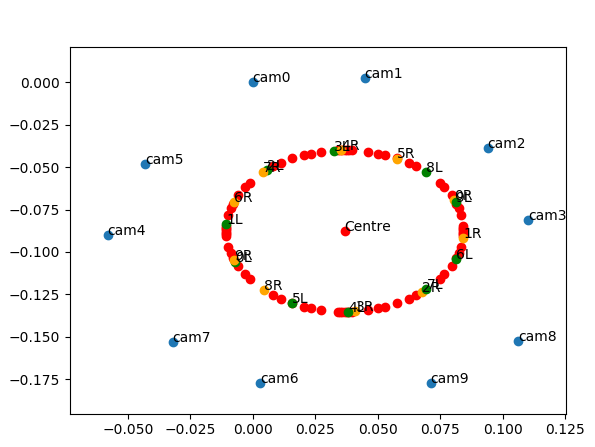
\includegraphics[width=0.8\linewidth]{pictures/our_camera_rig.PNG}
\end{center}
   \caption{An illustration of our camera rig based on the calibration file.}
\label{rig}
\end{figure}

\subsection{Flow estimation}
We did not implement such a sophisticated flow estimation algorithm as in Anderson et al.~\cite{jump16}. Instead, we used an existing per-pixel flow computation method from the OpenCV library.

\subsection{Exposure correction}
For the exposure correction, we interpolate linearly between the average image intensity of the neighboring image pairs:\\
\\
$g_{c}=\dfrac{(\theta_{c}-\theta_{0})}{(\theta_1-\theta_{0})}*g_{0} + \dfrac{(\theta_{1}-\theta_{c})}{(\theta_1-\theta_{0})}*g_{1}$
\\
\subsection{View interpolation}
The main idea of the stitching process is to interpolated between two neighboring images.
We used the following interpolation from Anderson et al.~\cite{jump16} for our view interpolation:\\
\\
$\theta_p=\dfrac{(\theta_{b}-\theta_{1})*\theta_{0}+(\theta_{0}-\theta_{a})*\theta_{1}}{\theta_{b}-\theta_{a}+\theta_{0}-\theta_{1}}$
\\
\\
Where $\theta_ {0}$ and $\theta_ {1}$ are the headings of the two cameras in the ODS stitch. $\theta_ {a}$ is the heading of a point in the first camera and $\theta_ {b}$ is the heading of the same point in the second camera (see figure\ref{interpolation}).

\begin{figure}[t]
\begin{center}
   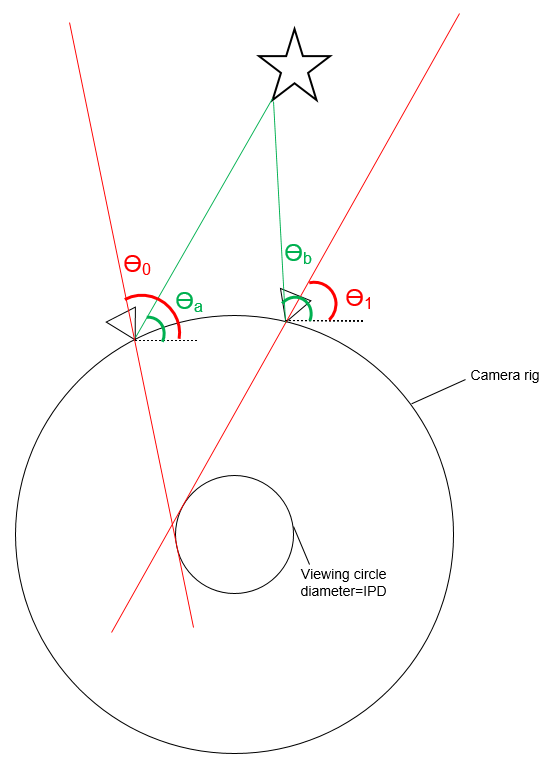
\includegraphics[width=0.7\linewidth]{pictures/interpolation.PNG}
\end{center}
   \caption{This is an illustration of the different angles used in the interpolation formula. The red lines are the central rays of the corresponding camera.}
\label{interpolation}
\end{figure}

\subsection{Stitching}



%------------------------------------------------------------------------
\section{Results}
For testing our implementation we used a dataset provided from our supervisor It's obtained from 10 cameras disposed on an ellipse approaching a circle, which are pairwise equidistant. The calibration file was provided too. For getting an idea of the possible output, we produced an homography stitching which can be seen in image ...
In Figure ~\ref{lefteye} we can instead see the output of the ODS stitching for our dataset for the left eye considering the first frame.
\begin{figure}[t]
\begin{center}
   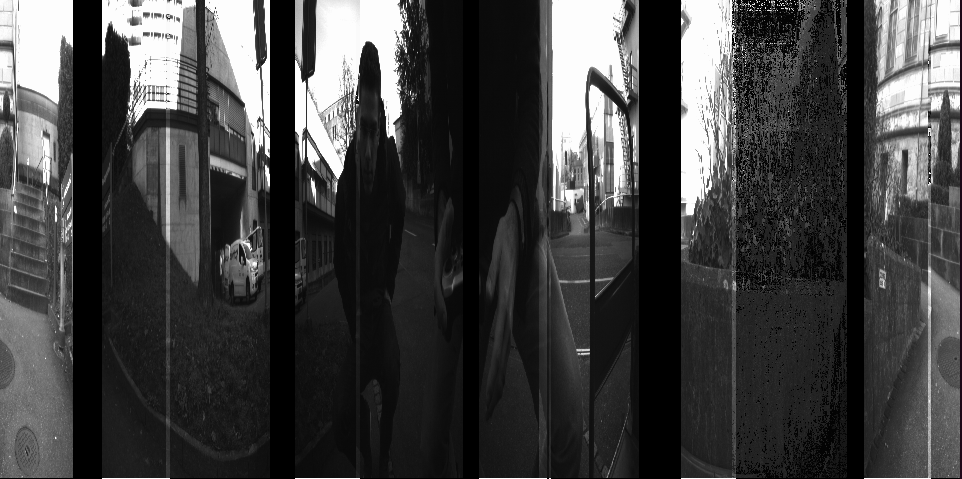
\includegraphics[width=0.7\linewidth]{pictures/frame0_lefteye_cwise.png}
\end{center}
   \caption{ODS stitching result for the left eye, first frame.}
\label{lefteye}
\end{figure}

%------------------------------------------------------------------------
\section{Discussion}
As we can see in picture ~\ref{lefteye} we get good results only for the camera couples which provide a good overlap. This is due to the fact that the optical flow between the other images is very low since they don't have much in common. Another issue is that if we take a look at the image planes plotted in Figure ~\ref{imageplanes} there are empty spaces between them. For this we don't have a real idea of why it happens, it could be because of problems with the calibration file.
Further, better results could have been obtained if we had an Odyssey GoPro at disposal since this would have given us the same working conditions as the authors had.
\begin{figure}[t]
\begin{center}
   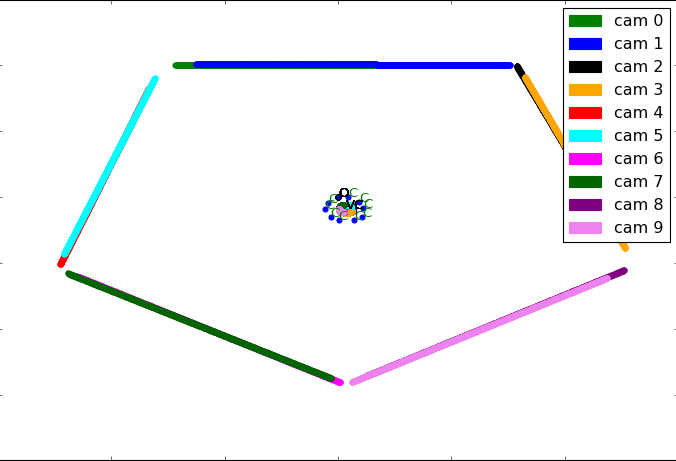
\includegraphics[width=0.7\linewidth]{pictures/rig_detailed.png}
\end{center}
   \caption{Plot of the image planes of the different cameras}
\label{imageplanes}
\end{figure}
%------------------------------------------------------------------------
\section{Conclusion}
The results obtained from Anderson et al.~\cite{jump16} are better than ours but this was expected. We had less cameras at disposal (10 instead of 16) which weren't in a perfect rig like it's the case using the Odyssey GoPro. This would have produced in general a better overlap among the images, which would have resulted in a better interpolation.

{\small
\bibliographystyle{ieee}
\bibliography{egbib}
}

\end{document}
